\section{Introduction}
Ambient noise—particularly in the form of broadband sound such as white, pink, or brown noise—has been widely used for decades to aid in relaxation, concentration, and sleep. These noise types differ in their spectral properties: white noise contains equal energy per hertz across the entire frequency spectrum, pink noise emphasizes lower frequencies with equal energy per octave, and brown noise (also known as Brownian or red noise) further intensifies low-frequency components, creating a deeper, more soothing sound. Despite their widespread use, the process of selecting the optimal noise type and fine-tuning its characteristics—such as volume, spectral balance, and texture—is typically subjective, inconsistent, and labor-intensive.

Moreover, the human brain responds to auditory stimuli in highly individualized and context-dependent ways. A particular noise profile that enhances relaxation for one person may be ineffective or even distracting for another. Additionally, even within the same individual, the optimal auditory stimulus can vary depending on time of day, cognitive load, emotional state, and environmental context. Traditional static noise generators do not account for these dynamic physiological and psychological variables, resulting in suboptimal or inconsistent outcomes.

The Neuro-Adaptive NoiseScape system addresses these limitations by introducing a closed-loop, neurofeedback-based approach to noise generation. This system integrates real-time electroencephalography (EEG) monitoring with adaptive audio synthesis algorithms to create a responsive sound environment. By continuously analyzing the user’s brainwave activity—such as alpha (8–12 Hz), beta (13–30 Hz), and theta (4–7 Hz) rhythms, which are associated with different mental states—the system infers the user’s current level of relaxation or cognitive engagement. It then dynamically adjusts parameters of the noise being played, such as its spectral density, amplitude modulation, and frequency coloration, to promote the brain's progression toward a desired state (e.g., deep relaxation or sustained attention).

This neuroadaptive feedback loop transforms ambient noise from a static tool into an intelligent, responsive system that is both personalized and context-aware. By aligning auditory stimulation with real-time neural data, the Neuro-Adaptive NoiseScape provides a scientifically grounded and user-specific method for optimizing mental states, with potential applications in wellness, mental health, productivity, and sleep science.

\section{Theory}

An important foundation for understanding adaptive sound design lies in the neural correlates of mental states, as measured by electroencephalography (EEG). EEG captures brain activity in the form of electrical oscillations, which can be categorized into frequency bands that correlate with psychological states. For example, alpha waves (8–12 Hz) are associated with calm wakefulness, beta waves (13–30 Hz) with focused cognitive engagement, and theta waves (4–7 Hz) with drowsiness and meditative states \cite{klimesch1999}. By tracking these rhythms in real time, it becomes possible to infer an individual’s cognitive state and respond accordingly, laying the foundation for a neuroadaptive sound system.

This real-time responsiveness is grounded in the concept of closed-loop brain-computer interfaces (BCIs), which continuously sense neural activity and adapt stimuli to support or guide the brain toward a desired state. In a review by Sitaram et al. (2017), such closed-loop systems are shown to effectively enhance self-regulation, attention, and even clinical outcomes in disorders such as ADHD and depression \cite{sitaram2017}. Unlike open-loop systems, which act independently of user state, closed-loop designs enable dynamic and personalized adaptation—crucial for auditory environments aiming to optimize mental performance or rest.

A key mechanism through which sound can actively influence neural activity is auditory entrainment. Rhythmic auditory stimulation, such as binaural beats or amplitude-modulated tones, can synchronize neural oscillations with external rhythms. This synchronization has been shown to influence states of attention, relaxation, and sleep \cite{nozaradan2014}.

A significant contribution to the understanding of how auditory stimulation can modulate brain activity during sleep comes from Besedovsky et al. (2017). Their study employed a closed-loop auditory stimulation method synchronized with slow oscillations in the EEG to enhance deep sleep quality. The results demonstrated that such stimulation not only strengthened slow-wave sleep—a critical phase for physical restoration and memory consolidation—but also amplified markers related to the immune system's supportive functions \cite{besedovsky2017}. While their work primarily focuses on sleep physiology, it reinforces the broader concept that adaptive soundscapes can actively influence neural dynamics when coupled with real-time neurofeedback.

Another perspective is offered by stochastic resonance, a phenomenon in which a moderate level of noise can enhance the detection of weak neural signals. Söderlund et al. (2010) found that children with attention deficits performed better on memory tasks when white noise was introduced—highlighting that noise can act as a cognitive enhancer under specific neurological conditions \cite{soderlund2010}. This finding supports the hypothesis that adaptive noise, when matched to individual brain dynamics, could benefit cognitive functioning in both clinical and non-clinical populations.

Given the interindividual variability in auditory processing and neural response, personalization is not a luxury but a necessity in effective sound-based interventions. By leveraging machine learning techniques alongside EEG data, a noise generation system can be trained to detect and respond to subtle changes in the user’s state, adjusting spectral content, modulation, and texture to suit moment-to-moment needs.

Finally, the broader applications of neuroadaptive noise systems span domains such as productivity, mental health, education, and sleep science. As demonstrated in human-computer interaction research \cite{mark2016}, carefully tuned digital environments can reduce stress, enhance focus, and support cognitive recovery. A sound environment that adapts in real time to the brain’s needs could support deep work sessions, therapeutic interventions, or mindful rest in ways that static systems cannot.

Taken together, these theoretical foundations underscore the significance of integrating EEG-based feedback with adaptive audio systems. By doing so, ambient noise moves from being a passive background element to an intelligent, responsive tool for mental state optimization.




\section{Methodology}

This chapter outlines the methodological approach of the 	extit{NoiseScape} project, which aims to explore how different noise configurations affect the user’s mental state, specifically in terms of relaxation and focus. To achieve this, we developed a desktop application that integrates a brain-computer interface (BCI) device from OpenBCI and allows users to test various noise environments while recording their EEG data. The methodology combines principles from experimental psychology, neuroscience, and software engineering to create a structured system for data collection, analysis, and interpretation.

\subsection{Experimental Design}

The project was carried out in several iterative phases, beginning with the definition of project goals and technical requirements. The initial concept was to allow users to select a target mental state (relaxed or focused), expose them to different types of noise, and evaluate which configuration most effectively supports the desired state. The core metric for relaxation was defined as the power of alpha waves (8-12 Hz), commonly associated with calm and restful brain activity.

In the planning stage, we designed a structured experimental protocol. Each participant is guided through a series of tasks under controlled conditions. The relaxation task requires the user to close their eyes and relax or think about something calming for two minutes. This task is repeated under nine different auditory conditions: eight with different types and volumes of noise, and one silent baseline condition. The noise conditions include white, pink, brown, and green noise, each at two user-defined volume levels (low and high). These volume levels are not defined by precise decibels but by subjective user comfort, determined using sliders in the application interface.

\subsection{EEG Data Collection and Analysis}

EEG data is recorded using the OpenBCI headset and streamed via the 	exttt{openbci-python} library. The noise is generated using 	exttt{NumPy} and played back with the 	exttt{sounddevice} library. The EEG data is saved in labeled formats that correspond to the noise condition and task type. All data is stored in a structured directory path, which can be set by the user at the start of the experiment.

The data analysis is conducted offline. First, the EEG recordings are preprocessed using Python. Bandpass filtering (typically 0.5-50 Hz) is applied with 	exttt{SciPy} to remove noise outside the relevant EEG bands. Artifacts such as eye blinks may optionally be removed, though this step can be skipped for simplification. Alpha power is then calculated using spectral analysis methods like Fourier transforms or Welch’s method. The sum of power in the alpha band (8-12 Hz) is computed for each condition.

The main analytical goal is to compare alpha power across all conditions. By examining which noise condition results in the highest alpha power relative to the baseline, we can infer which noise setup best supports relaxation or focus. Trends in the data are visualized using bar plots, created with libraries such as 	exttt{Matplotlib}, showing the alpha power for each condition.






\section{Application}

\subsection{System Architecture and Technologies}

The development of \textit{NoiseScape} followed a parallel path to the experiment design. Built using \texttt{Electron} with a \texttt{Node.js} backend, the desktop application runs on both macOS and Windows and is designed to guide users through the study in a structured and interactive way.

\begin{itemize}
\item \textbf{EEG Interface}: Streams real-time data from an OpenBCI device using \texttt{openbci-python}.
\item \textbf{Noise Engine}: Generates broadband noise using \texttt{NumPy} and plays it via \texttt{sounddevice}.
\item \textbf{Data Logging}: Stores EEG recordings and associated condition metadata in structured directories for later analysis.
\end{itemize}

\subsection{Graphical User Interface (GUI)}

The GUI is divided into three equally sized vertical panels and a bottom control row spanning the entire width, as well as a footer. The design follows a modern flat aesthetic with a dark grey background, bold white fonts, white-bordered elements, and soft border radii.

\begin{itemize}
\item \textbf{Left \textendash{} EEG Frequency Bands}: Displays real-time power across the five standard EEG bands: Delta, Theta, Alpha, Beta, and Gamma. Each band is represented visually with bold white fonts and waveforms within bordered boxes.

\item \textbf{Center \textendash{} Noise Sound (Free Play Mode)}: Features a visual audio spectrum analyzer (20 Hz\textendash{}20 kHz) with ten vertical rainbow-colored sliders (from red to pink). These allow manual spectral shaping of noise, all sliders defaulting to a neutral center. Below the sliders:
\begin{itemize}
\item A white horizontal volume slider (range 1\textendash{}9) with a circular knob, curved border, and visual indication of volume.
\item A section titled \textbf{Defined Volumes} with three identical sliders labeled Low, Middle, and High. These are reference points for subjective volume perception and do not influence playback.
\item A section titled \textbf{Adaptive Noise Sound} (in turquoise). Below it, a turquoise Play button becomes active only once all study conditions and baseline data have been logged. This feature plays the best noise configuration based on EEG patterns (e.g., highest alpha activity for the selected state).
\end{itemize}

\item \textbf{Right \textendash{} Study Mode}: Contains nine pre-configured buttons grouped by noise type and volume level:
\begin{itemize}
\item \textbf{White Noise (white)}: Low, Middle, High
\item \textbf{Right-Skewed Noise (modern red)}: Emphasizes lower frequencies (slider ramp from red high to pink low).
\item \textbf{Left-Skewed Noise (modern pink)}: Emphasizes higher frequencies (slider ramp from pink high to red low).
\end{itemize}
Each button triggers a specific preset, starts the corresponding playback, and enables logging of EEG data with metadata.
\end{itemize}

The \textbf{bottom control row} includes:
\begin{itemize}
\item \textbf{Bottom Left}:
\begin{itemize}
\item \textbf{Set Root Path}: Opens a dialog for selecting the base directory for logs.
\item \textbf{Select State to Achieve}: A dropdown labeled \textit{State to Achieve} (currently only: Relaxed).
\end{itemize}
\item \textbf{Bottom Right}:
\begin{itemize}
\item \textbf{Log EEG + NO Noise} (black button): Starts a 2-minute EEG recording only if no noise is currently playing. Saves EEG as baseline.
\item \textbf{Log EEG + Noise} (green button): Records EEG and noise metadata for 2 minutes, only enabled if one of the study mode buttons is active.
\end{itemize}
\end{itemize}

\begin{figure}[H]
\centering
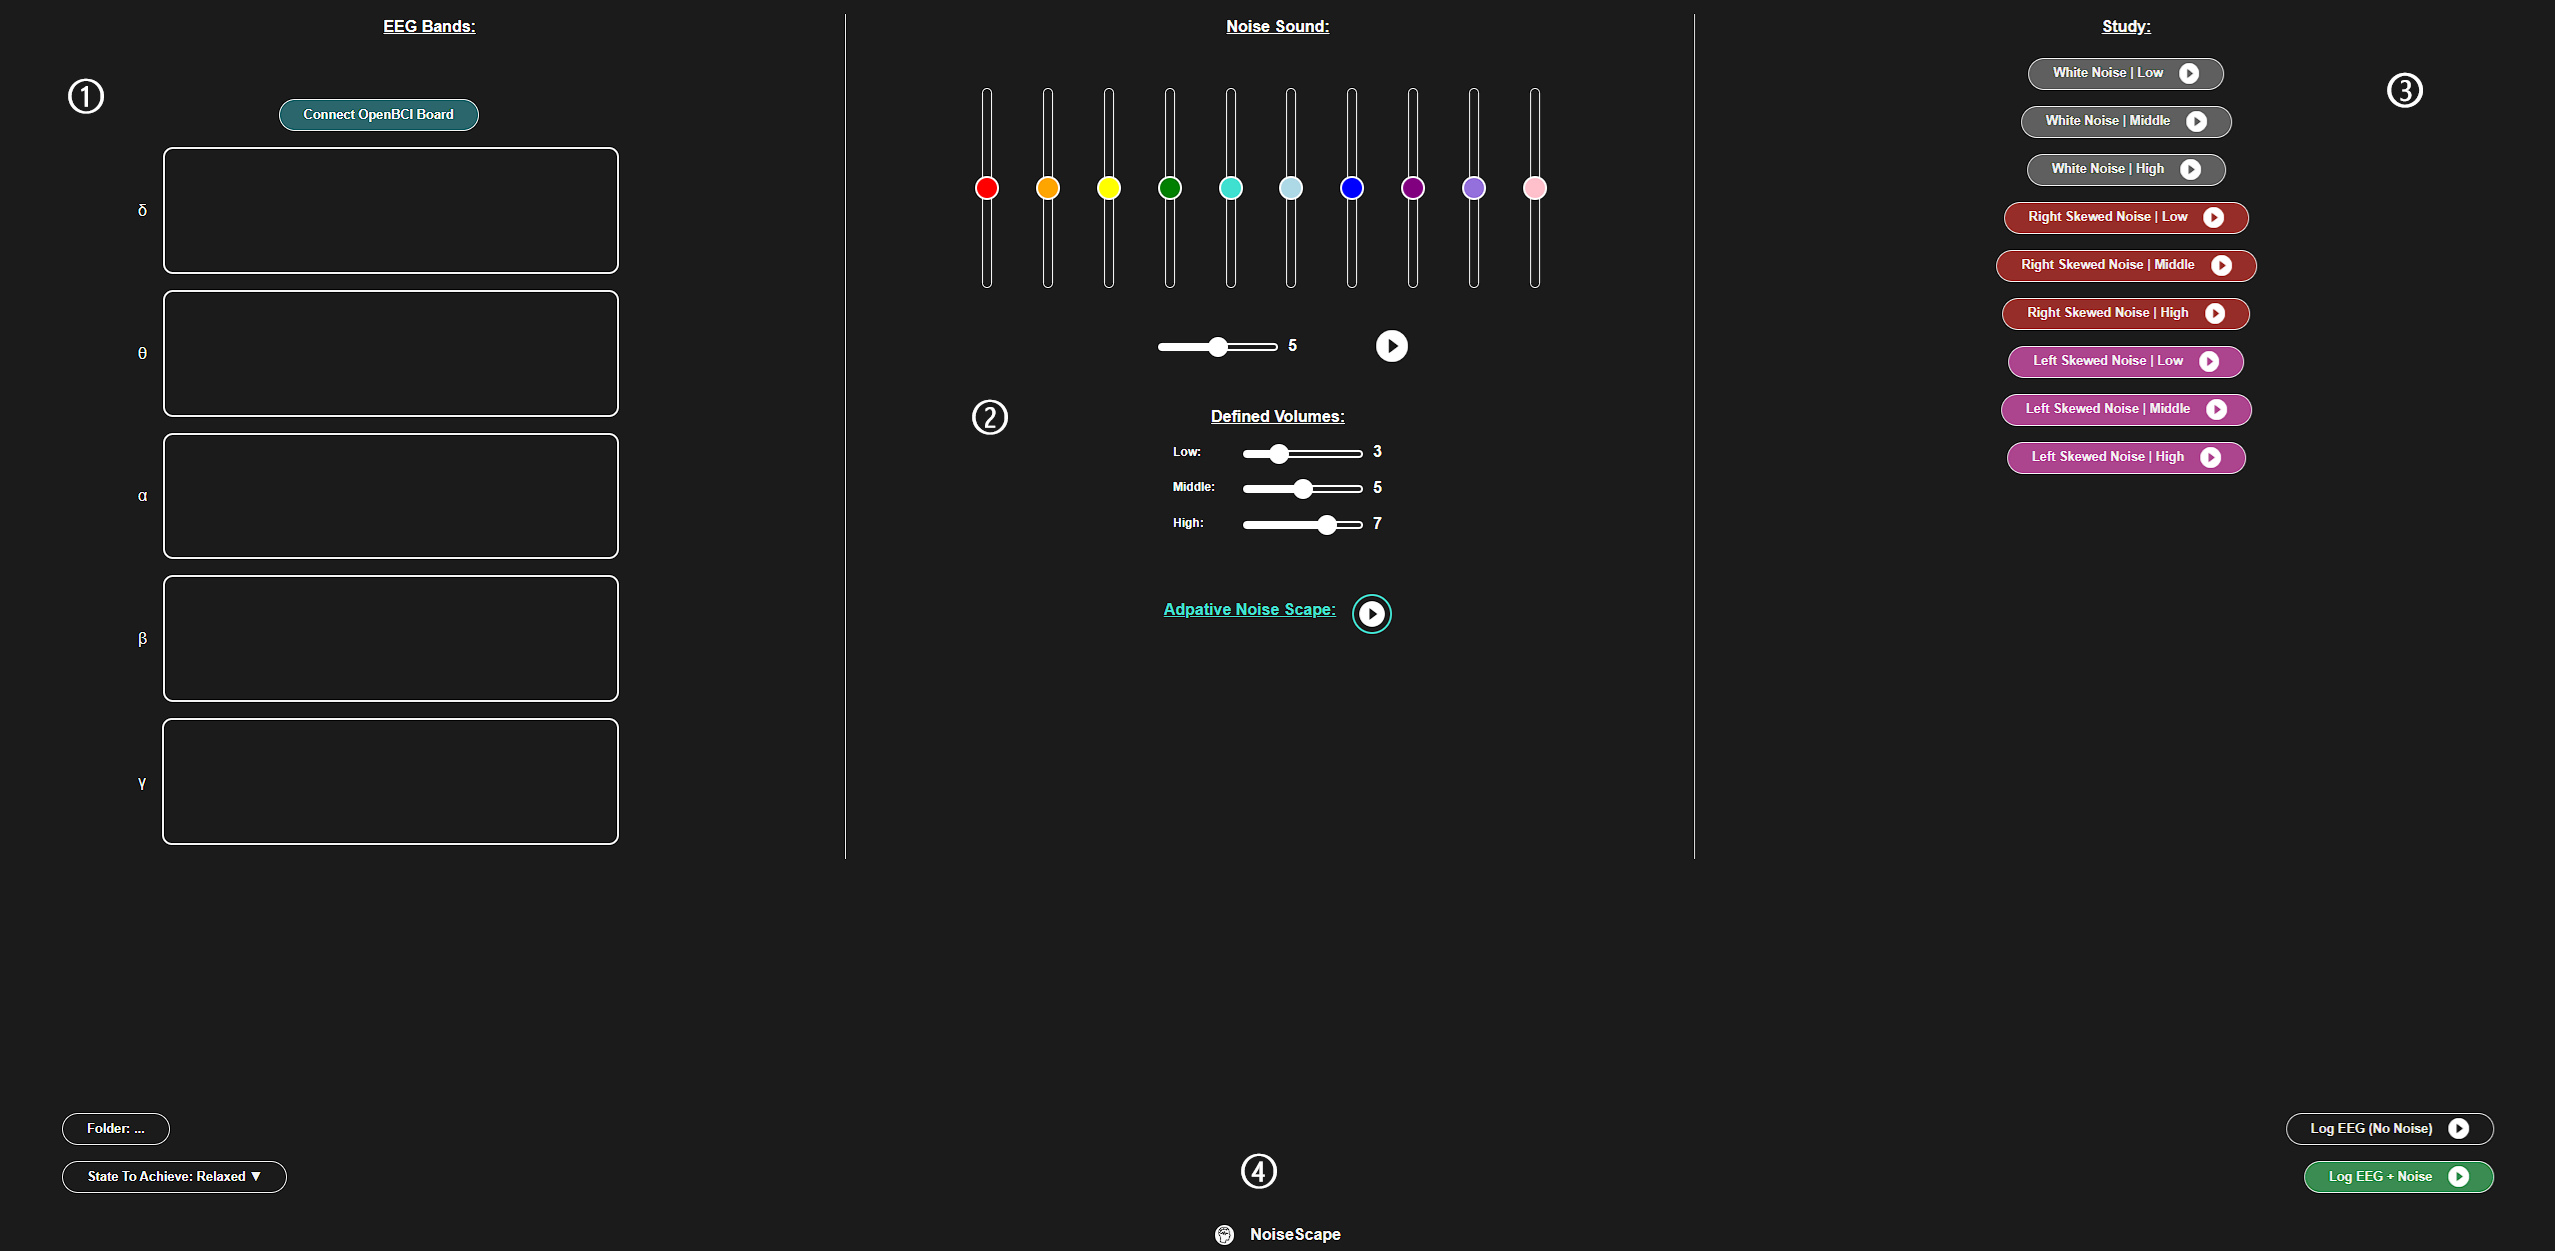
\includegraphics[width=0.5\textwidth]{interface.png}
\caption{Graphical user interface of the NoiseScape application.}
\end{figure}


Noise profiles are derived from raw white noise shaped using slider presets:

\begin{itemize}
\item \textbf{White Noise}: All sliders centered to produce a flat frequency spectrum.
\item \textbf{Right-Skewed Noise}: Linearly emphasizes lower frequencies by gradually lowering slider values from left to right.
\item \textbf{Left-Skewed Noise}: Linearly emphasizes higher frequencies by raising slider values from left to right.
\end{itemize}

When a study condition is activated, playback is updated with the respective configuration, and EEG data is saved with a descriptive label (e.g., \texttt{pink\_high}, \texttt{white\_low}, \texttt{baseline}).

The Adaptive Noise button uses previously collected EEG data to select or interpolate a configuration that best aligns with the desired mental state (e.g., Relaxed).











\section{Discussion and Future Work}

NoiseScape demonstrates the feasibility of integrating EEG measurement with interactive sound environments in a structured experimental setting. Its modular architecture and intuitive interface make it suitable for both protocol-driven trials and exploratory usage.

A key current limitation is the absence of real-time adaptation. While the system identifies optimal configurations through offline analysis, it does not yet dynamically adjust noise during a session. However, its design readily supports future enhancements such as:

\begin{itemize}
\item \textbf{Live EEG Classification}: Incorporating lightweight machine learning models (e.g., SVM, k-NN) to infer mental state in real time.
\item \textbf{Expanded Mental States}: Supporting additional states such as focused attention (beta activity) or meditative/drowsy states (theta).
\item \textbf{Multimodal Sensing}: Integrating heart rate variability (HRV), galvanic skin response (GSR), or respiration to improve state detection accuracy.
\item \textbf{Immersive Environments}: Extending the system to VR headsets or mobile platforms with embedded EEG.
\item \textbf{Open Dataset}: Publishing anonymized EEG-noise data to foster reproducibility and facilitate benchmarking in auditory neurofeedback research.
\end{itemize}

These extensions would enable NoiseScape to evolve from an experimental research tool into a fully adaptive, real-time neurofeedback platform with broad applicability in wellness, cognitive enhancement, and human-computer interaction.








\section{Conclusion}

NoiseScape offers a structured and scalable environment for investigating how different types and configurations of ambient noise influence brain activity. By combining real-time EEG streaming, flexible noise playback, and structured data logging, the system enables empirical discovery of auditory setups that best support mental relaxation.

Although the current version is limited to offline analysis, the underlying architecture is designed for future extensions, including real-time neuroadaptive feedback. As such, NoiseScape lays a practical and conceptual foundation for intelligent sound environments tailored to the listener’s neural state.

%\begin{figure}\[h]
%\centering
%\fbox{\includegraphics\[width=0.7\linewidth]{figures/pilot\_results\_placeholder.png}}
%\caption{Example plot of alpha power across different noise conditions. (To be added after pilot data collection.)}
%\label{fig\:pilot\_results}
%\end{figure}